\documentclass[10pt,letterpaper]{article}
\usepackage[top=1in,bottom=1in,left=1in,right=1in]{geometry}
\usepackage{datetime}
\usepackage{natbib}      % http://merkel.zoneo.net/Latex/natbib.php
\usepackage{palatino}
\usepackage{verbatim}
\usepackage[normalem]{ulem}
\bibpunct{(}{)}{;}{a}{,}{,}

\usepackage{array}

\usepackage{chngpage}
\usepackage{stmaryrd}
\usepackage{amssymb}
\usepackage{amsmath}
\usepackage{graphicx}
\usepackage{lscape}
\usepackage{subfigure}
\usepackage[usenames,dvipsnames]{color}
\definecolor{myblue}{rgb}{0,0.1,0.6}
\definecolor{mygreen}{rgb}{0,0.3,0.1}
\usepackage[colorlinks=true,linkcolor=black,citecolor=mygreen,urlcolor=myblue]{hyperref}

\setlength{\tabcolsep}{12pt}


\newcommand{\bocomment}[1]{\textcolor{Bittersweet}{BO says: #1}}

\newcommand{\inner}[1]{\langle #1 \rangle} 
\newcommand{\smallsec}[1]{\noindent \textbf{#1\ }}
\newcommand{\cmd}[1] {{\color{blue}\texttt{#1}}}

\newcommand{\solution}[1]{{\color{myblue} \emph{[Solution:} 

#1 

\emph{End solution]}}}
\newcommand{\solutionnote}[1]{{\color{myblue} \emph{[Note:}

#1 

\emph{End note]}}}
\newcommand{\points}[1]{{\color{mygreen}\emph{[#1]\ \ }}}

\newcommand{\aone}{\diamondsuit}
\newcommand{\atwo}{\heartsuit}
\newcommand{\bone}{\triangle}
\newcommand{\btwo}{\Box}
\newcommand{\myand}{\ \land\ }
\newcommand{\myor}{\ \lor\ }
\newcommand{\mynot}{\lnot}

\title{
  \textbf{Mini-project 3} \\
  \Large{CMPSCI 670, Fall 2019, UMass Amherst} \\
  \Large{Instructor: Subhransu Maji} \\
  \Large{TAs: Aruni RoyChowdhury, Archan Ray}
}

\settimeformat{ampmtime}
\date{}
\begin{document}
\maketitle

\renewcommand\thesubsection{\thesection.\alph{subsection}}


\section*{Guidelines}

\paragraph{Submission.} Submit a \emph{single pdf document} via moodle that includes your solutions, figures and code. The latex source file for the homework is provided which you can modify to produce your report. You are welcome to use other typesetting software as long as the final output is a pdf. For readability you may attach the code printouts at the end of the solutions within the same pdf. Note that we will not run your code. Similarly figures should be included in a manner which makes it easy to compare various approaches. Poorly written or formatted reports will make it harder for the TA to evaluate it and may lead to a partial deduction of credit. 

\paragraph{Late policy.} You could have 24 hours late submission with a 50\% mark down. Late submission beyond 24 hours will not be given \emph{any} credits.

\paragraph{Plagiarism.} We might reuse problem set questions from previous years, covered by papers and webpages, we expect the students not to copy, refer to, or look at the solutions in preparing their answers. We expect students to want to learn and not google for answers. 

\paragraph{Collaboration.} The homework must be done individually, except where otherwise noted in the assignments. 'Individually' means each student must hand in their own answers, and each student must write their own code in the programming part of the assignment. It is acceptable, however, for students to collaborate in figuring out answers and helping each other solve the problems. We will be assuming that you will be taking the responsibility to make sure you personally understand the solution to any work arising from such a collaboration.

\paragraph{Using other programming languages.} We made the starter code available in Python and Matlab. You are free to use other languages such as Octave or Julia with the caveat that we won't be able to answer or debug non Matlab/Python questions.

\paragraph{Python requirements.} We will be using Python 2.7. The Python starter code requires \cmd{scipy}, \cmd{numpy} (at least v1.12), and \cmd{scikit-image}.
If you are not familiar with installing those libraries through some package manager (like \cmd{pip}), the easiest way of using them is installing \href{https://conda.io/docs/user-guide/install/index.html}{Anaconda}.


\newpage

\section{Image denoising [35 points]}
In this part of the homework you will evaluate two simple denoising algorithms, namely Gaussian filtering and median filtering. In addition you will also implement a more advanced algorithm based on non-local means. The starter code for this part is in \cmd{evalDenoising}. The test images are provided in the \cmd{data/denoising} folder. There are five images:
\begin{itemize}
\item \texttt{saturn.png} -- noise-free image for reference
\item \texttt{ssaturn-noise1g.png, saturn-noise2g.png}  -- two images with i.i.d. Gaussian noise 
\item \texttt{ssaturn-noise1sp.png, saturn-noise2sp.png}  -- two images with ``Salt and Pepper" noise
\end{itemize}
The two images correspond to different amounts of noise. The \cmd{evalDenoising} script loads three images, visualizes them, and computes the error (squared-distance) between them as shown below. Your goal is to denoise the images which should result in a lower error value. 

\begin{figure}[h]
\centering
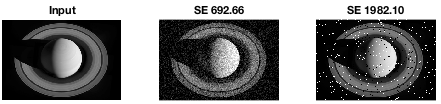
\includegraphics[width=0.8\linewidth]{denoising-output.png}
\caption{\label{fig:denoising} Input images for denoising.}
\end{figure}

\begin{itemize}
  \item \points{5 points} Using Matlab's \cmd{imfilter} function, implement a Gaussian filter. You may find the function \cmd{fspecial} useful to create a Gaussian kernel. In Python, you can use the function \cmd{convolve} from \cmd{scipy.ndimage.filters}. Additionally, we added a function \cmd{gaussian} to \cmd{utils.py} that does the same as \cmd{fspecial('gaussian')}. Experiment with different values of the standard deviation parameter $\sigma$. Report the optimal error and $\sigma$ for each of these images.
  \item \points{5 points} Using Matlab's \cmd{medfilt2} function, implement a median filter. In Python, you can use \cmd{medfilt2} from \cmd{scipy.signal}. Report the optimal error and neighborhood size for each of the images.
\item \points{20 points} Implement a function to compute non-local means filtering. Recall that for each pixel in the input image the algorithm computes the denoised value as weighted mean of all the pixel values within the window, where the weight is some inverse function of the distance between patches centered at the pixels.

Let $I(x)$ denote the pixel value at $x$, $\hat{I}(x)$ denote the pixel value after denoising, $P(x)$ denote the patch of radius p centered around $x$, and $W(x)$ denote the pixels within a window of radius w around $x$. One choice of weight function is a Gaussian with a paramter ($\gamma$) resulting in the following update equation for each pixel:


\begin{equation}
\hat{I}(x) = \frac{\sum_{y \in W(x)}\exp\{-\gamma||P(x) - P(y)||^2_2\}I(y)}
{\sum_{y \in W(x)} \exp\{-\gamma||P(x) - P(y)||^2_2\}}.
\end{equation}
Here $||x||^2_2$ denotes the squared length of the vector $x$. Write a function to implement this operation. Your function should take as input the noisy image, a patch radius (p), window radius (w), and a bandwidth parameter $\gamma$ and return denoised image.

This algorithm is slower in comparison to the local-filtering based approaches since it involves pairwise distance computations to all pixels within each neighborhood. My implementation takes about 15 seconds for a patch size of 5x5 and neighborhood size of 21x21.
I suggest debugging your algorithm and find the range of parameters that work well on a smaller crop of the image before trying it on the full image. 
Experiment with different values of the parameters and report the optimal ones and the corresponding errors for each of the images. Include your implementation in the submission.

\item \points{5 points} Qualitatively compare the outputs of these results. You should include the outputs of the algorithms side-by-side for an easy comparison. Which algorithm works the best for which image? 
\end{itemize}



\section{Texture synthesis [30 points]}

In this part you will implement various methods synthesizing textures
from a source image.


\begin{figure}[h]
\centering     
\begin{tabular}{cc}
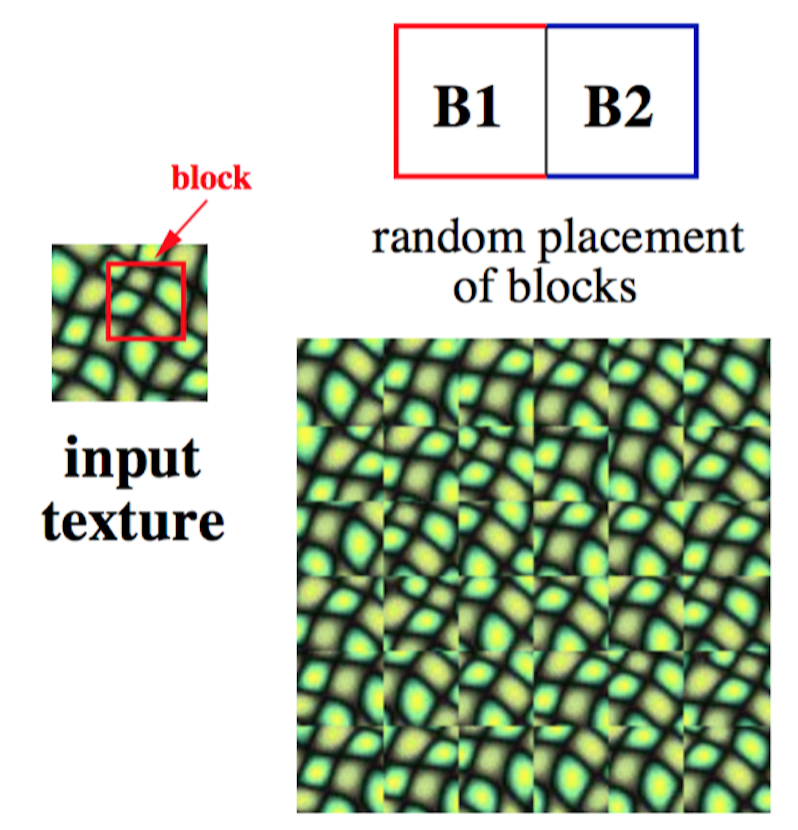
\includegraphics[width=0.25\linewidth]{random-patches.png} & 
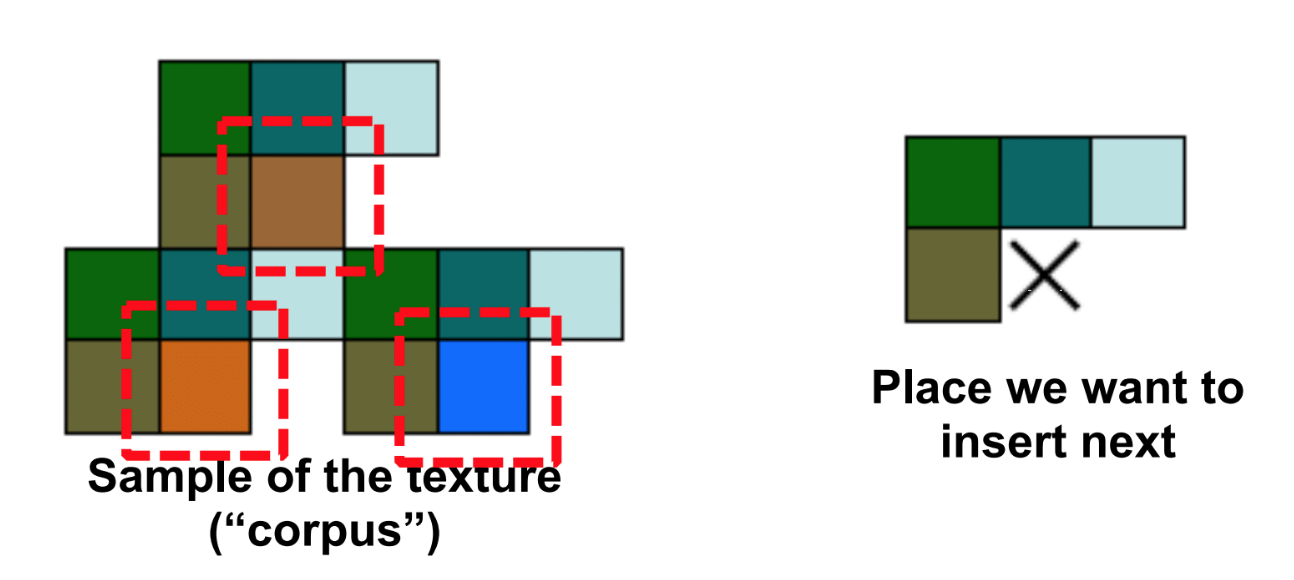
\includegraphics[width=0.5\linewidth]{pixel_neighbor.png} \\ 
(a) Random tiling & (b) Non-parametric sampling \\
\end{tabular}

\caption{\label{fig:image-synth} (a) Creating an output image by
  randomly picking patches from a source image. (b) Generating an
  output image pixel (\textit{right}) based on its neighbors in the
  source image (\textit{left}) (from lecture slides). In this example,
  the output pixel is likely to get a blue color.}

\end{figure}

\begin{itemize}
\item \points{5 points}  A simple approach for generating a texture is
  to randomly tile the target image using patches from a source
  image, as seen in Figure~\ref{fig:image-synth}(a). The basic
  procedure is as follows:

\begin{enumerate}
   \item Initialize an empty output image.
   \item Pick a tile randomly from the source image and copy into the
     output image at the top-left position.
   \item Proceed to the next unfilled position in the output image in
     raster order (left-to-right, top-to-bottom).
\end{enumerate}

Your output images should consist of $5 \times 5$ tiles; try various
tile sizes -- 15, 20, 30, 40. 
Use grayscale versions of the three images provided in the
\cmd{data/texture} folder.
 

\item \points{25 points} The above method results in an image with artifacts around the edge of the tiles. This is because the tiles do not align well.
  The approach of Efros and Leung avoids this by generating the ouput,
  one pixel at a time, by matching the local neighborhood
  of the pixel in the generated image and source image, as shown in
  Figure~\ref{fig:image-synth}(b).
The basic approach is summarized as follows:
 \begin{enumerate}
   \item Initialize an empty output image.
   \item Pick a $3 \times 3$ seed patch randomly from the source image
     and copy into the output image at the center position. The output
     image is generated by growing the borders of the filled pixels in
     the output image.
   \item Create a list of pixel positions in the output image that are
     unfilled, but contain filled pixels in their neighbourhood
     (\cmd{pixelList}). 
   \item Randomly permute the list and then sort by the number of
     filled neighbourhood pixels.
   \item For each pixel in \cmd{pixelList}, get a \cmd{ValidMask} for
     its neighbourhood. This would be a $windowSize \times windowSize$
     kernel, with 0s for unfilled positions and 1s at the
     neighbourhood positions of that pixel that contain filled
     pixels. Note, all this is done using the \textit{output} image.
   \item Compute the sum of squared differences (SSD) between every
     patch in the \textit{input} image w.r.t. the current unfilled
     pixel in the \textit{output} image. Take care to ensure the
     \cmd{ValidMask} is applied when computing the SSD --- we want to
     find the pixels in the input image have a similar neighbourhood
     w.r.t. the \textit{filled} neighbours of the currently unfilled
     pixel in the output image.
   \item Calculate \cmd{minSSD}, which is the smallest distance among
     all input image pixel neighbourhoods to the current output
     pixel's neighbourhood.
   \item Select a list of \cmd{BestMatches}, which are input image
     pixels within \texttt{minSSD*(1+ErrThreshold)}, where
     \cmd{ErrThreshold} is set to 0.1.
   \item Randomly pick an input image pixel from \cmd{BestMatches} and
     paste its pixel value into the current unfilled output pixel
     location.
   \item Keep repeating the steps for creating \cmd{pixelList} with
     unfilled output image locations, until all unfilled positions are
     filled. 
\end{enumerate}

Not all these steps need to implemented exactly. For instance, you
could come up with other strategies on how to grow the texture (e.g., grow the border
systematically by going clockwise from the top-left corner.).

The starter code for this part is in \cmd{evalTextureSynth}. The
source textures are in the \cmd{data/texture} folder (Note that
there are three).
Your goal is to implement the texture synthesis algorithm so that for
each small image provided, starting from a $3 \times 3$ seed patch,
you are able to generate a $70 \times 70$ image. 
For this homework you should convert the input
images to grayscale for faster processing.
Show the effect of various window sizes -- 5, 7, 11, 15. 
Discuss the effect of window size on runtime and synthesis quality. 



\section{Report writing and presentation [10 points]}

Please follow the guidelines for writing a good report.
Graders will penalize reports that are poorly written and fail to present the results in a reasonable manner.



\section{Extra credit [10 points]}
Here are some ideas for extra credit. 

\begin{enumerate}

\item \textbf{Block Matching 3D (BM3D).} The non-local means algorithm
  takes the weighted mean of the patches within a
  neighborhood. However there are other sophisticated approaches for
  estimating the pixel values. One such approach is BM3D
  (\url{http://www.cs.tut.fi/~foi/GCF-BM3D/}) which estimates the
  pixel value using a sparse basis reconstruction of the
  blocks. Compare an implementation of this approach to the non-local
  means algorithm.

\item \textbf{Image quilting.} The random tiling approach works
  reasonably well for some textures and is much faster than the
  pixel-by-pixel synthesis approach. 
  However, it may have visible artifacts at the border. 
  The ``Image Quilting'' approach from Efros and Freeman, proposes a
  way to minimize these by picking tiles that align well along the
  boundary (like solving a jigsaw puzzle).
  The basic idea is to pick a tile that has small SSD along the
  overlapping boundary with the tiles generated so far, as seen in Figure~\ref{fig:quilt}.
  An extention is to carve a ``seam'' along the boundary which
  minimizes this error further, which can be solved using dynamic programming. 
  The basic procedure (without seam carving) is as follows:
\begin{enumerate}
  \item Initialize an empty output image and copy a random tile from source image to the top-left corner
  \item Define the size of the region of overlap between tiles -- typically 1/6.
  \item Find SSD (sum of squared difference) between the neighbors of the output image tile position and each tile position in the source image, considering the region of overlap
  \item Find the tile in source image with lowest SSD (\texttt{minSSD}) with respect to the current tile in output image
  \item Make a list of all other tiles in the source image within a tolerance of the best tile's SSD (within \texttt{(1 + errTol) * minSSD}). 
\item Pick a tile randomly from the above list and copy into the output image
\item Proceed to the next un-filled position in the output image (left-to-right, top-to-bottom)
\end{enumerate}

Take a look at the paper for details:
  \url{http://www.cs.berkeley.edu/~efros/research/quilting.html}.

\begin{figure}
\centering
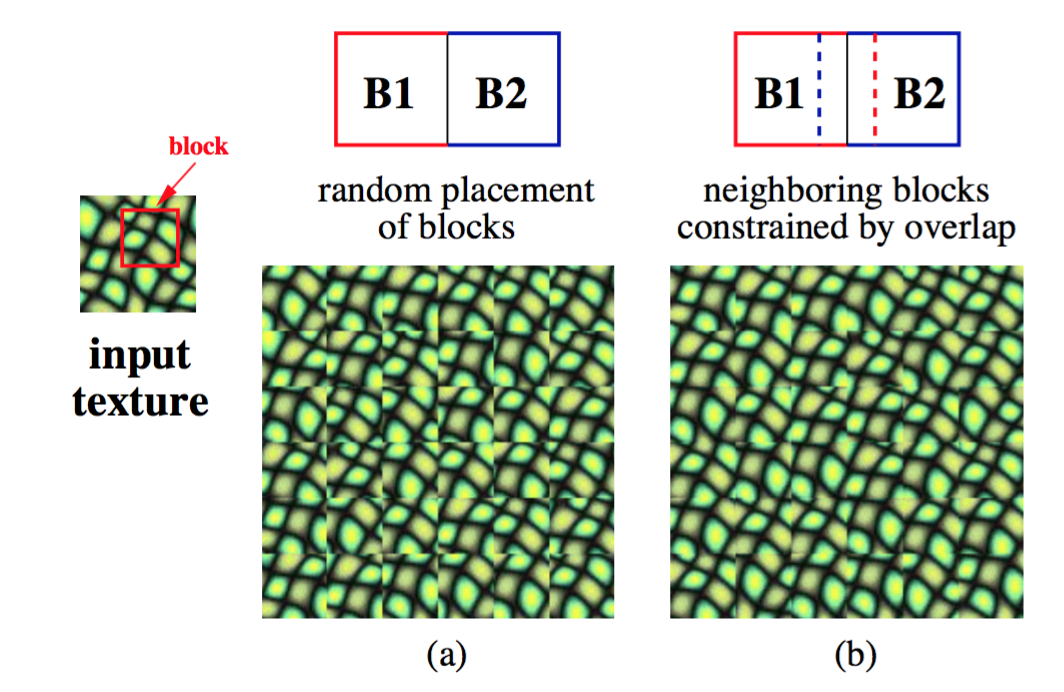
\includegraphics[width=0.6\linewidth]{image_quilt_fig.png}
\caption{\label{fig:quilt} Image quilting. Figure source:
  \url{https://people.eecs.berkeley.edu/~efros/research/quilting.html}.}
\end{figure}



\end{enumerate}
\end{itemize}


\end{document}
